\section{Motivation}\label{sec:2:motivation}

The shift from fine-granular predictive process forecasting including best next-step, remaining time prediction, and goal-oriented prediction to model-based prediction allows to obtain new insights into the global development of the process.
Consider the example in Figure \ref{fig:dfg_example_intro} where the road fine traffic management event log\footnote{\url{https://doi.org/10.4121/uuid:270fd440-1057-4fb9-89a9-b699b47990f5}} is partitioned into 100 intervals in which an equal number of DF relations occur.
\begin{figure}
    \centering
    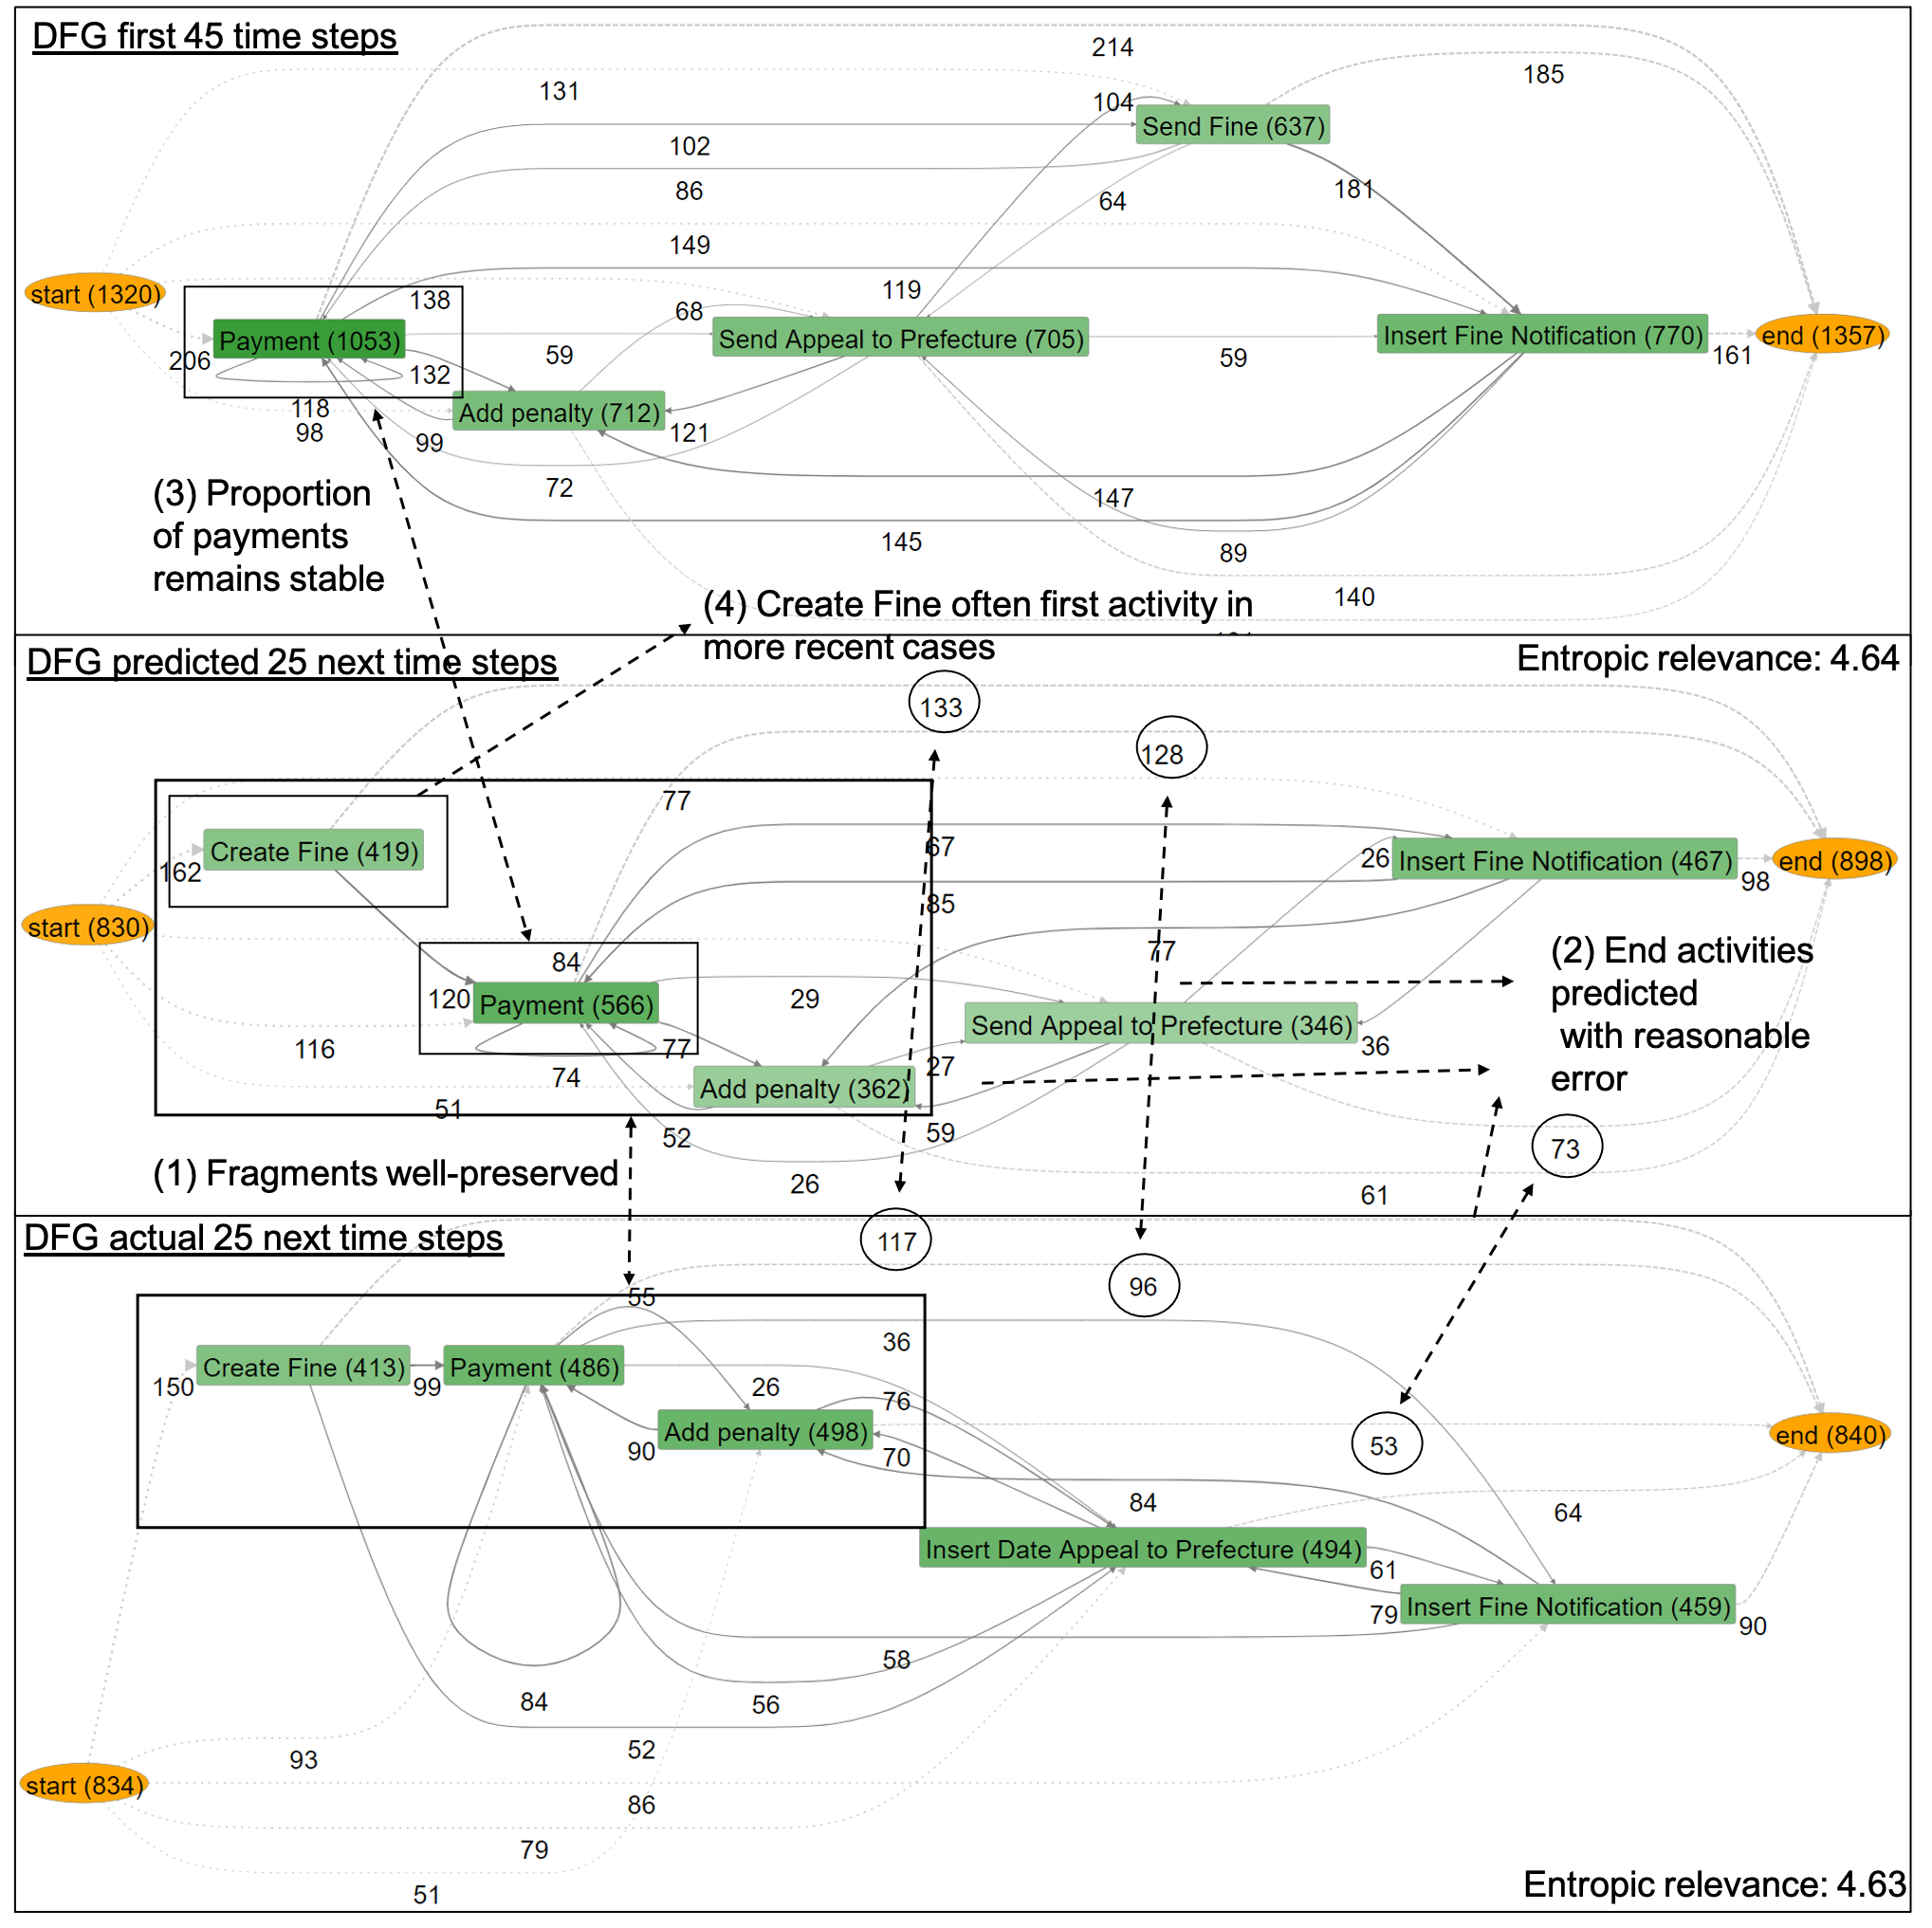
\includegraphics[width=0.85\textwidth]{img/MotExample2.png}
    \caption{Directly-follows graphs of the 45 first intervals of the event log, as well as a forecasted and actual DFG of the 25 next intervals.}
    \label{fig:dfg_example_intro}
\end{figure}
The DFs in the first 45 intervals are used to predict the final 25 intervals.
Entropic relevance \cite{DBLP:conf/icpm/PolyvyanyyMG20} is used to indicate that both the predicted and actual DFGs are of similar quality in terms of conformance (see Section \ref{sec:experiment}).
The DFGs show how process model forecasting and change exploration can provide multiple unique insights at a glance:
\begin{enumerate}
    \item The fragments and arc weights of the DFGs are well-preserved in the forecasted model;
    \item The end activities are predicted with reasonable accuracy (+/- 10\%);
    \item Compared to the initial 45 intervals the proportion of fine payments stays stable;
    \item The \emph{Create Fine} activity appears as a start activity more often - indicating a possible process drift.
\end{enumerate}
These provide insight both in terms of the past en present model ((3)-(4)) and the quality of forecasts between the actual and forecasted model ((1)-(2)).
Being able to construct such a predictions allows stakeholders to make estimates regarding how the overall fine system will evolve and allows to answer questions such as `How many more fines will be received?', `Will the backlog of fines be reduced?', `Will all fines be paid', and `Will the ratio of unpaid fines stay the same?'
This motivating example shows that where process mining/monitoring focuses on learning the as-is model to inform the to-be model and suggest potential repairs and improvements, process model forecasting allows to already grasp the future outcomes of the current as-is process which allows to shortcut potentially wrong outcomes \cite{DBLP:conf/bpm/PollPRRR18}.

Note that the horizon is longer compared with next-step prediction, and that these results would only be obtainable if long next-step predictions were performed.
Hence, both are complementary by their being used as varying horizons to obtain a full picture of the future development of a process (model).
Process model forecasting remains complementary with remaining time prediction as well, which could indicate what activities lead to what remaining time.
The process model forecast can partially assume goal-oriented prediction, as the forecast DFG allows to answer multiple oftentimes used goal statements pertaining to the execution of a particular activity, or a precedence relationship of a particular activity pair \cite{DBLP:journals/tkdd/TeinemaaDRM19} at the same time.
